%%% exemplo de utilização da classe ita
%%%
%%%   por        fábio fagundes silveira   -  ffs [at] ita [dot] br
%%%              benedito c. o. maciel     -  bcmaciel [at] ita [dot] br
%%%              giovani volnei meinertz   -  giovani [at] ita [dot] br
%%%    	         hudson alberto bode       -  bode [at] ita [dot]br
%%%    	         p. i. braga de queiroz    -  pi [at] ita [dot] br
%%%    	         jorge a. b. gripp         -  gripp [at] ita [dot] br
%%%    	         juliano monte-mor         -  jamontemor [at] yahoo [dot] com [dot] br
%%%    	         tarcisio a. b. gripp      -  tarcisio.gripp [at] gmail [dot] com
%%%
%%%   versão para overleaf:
%%%   por           alejandro a. rios cruz - aarc.88@gmail.com
%%%                 saulo gómez            - sagomezs@unal.edu.co
%%%  importante: o texto contido neste exemplo nao significa absolutamente nada.  :-)
%%%              o intuito aqui eh demonstrar os comandos criados na classe e suas
%%%              respectivas utilizacoes.
%%%
%%%  tese.tex  2016-08-25
%%%  $headurl: http://www.apgita.org.br/apgita/teses-e-latex.php $
%%%
%%% italus
%%% instituto tecnológico de aeronáutica --- ita, sao jose dos campos, brasil
%%%                   http://groups.yahoo.com/group/italus/
%%% discussion list: italus {at} yahoogroups.com
%%%
%++++++++++++++++++++++++++++++++++++++++++++++++++++++++++++++++++++++++++++++
% para alterar o tipo de documento, preencher a linha abaixo \documentclass[?]{?}
%   \documentclass[tg]{ita}			= trabalho de graduacao
%   \documentclass[tgfem]{ita}	= para engenheiras
%   								msc     		= dissertacao de mestrado
%   								mscfem   		= para mestras
%   								dsc      		= tese de doutorado
%   								dscfem   		= para doutoras
%   								quali    		= exame de qualificacao
%   								qualifem 		= exame de qualificacao para doutoras
% para 'draft version'/'versao preliminar' com data no rodape, adicionar 'dv':
%   \documentclass[dsc, dv]{ita}
% para trabalhos em inglês, adicionar 'eng':
%   \documentclass[dsc, eng]{ita}
%		\documentclass[dsc, eng, dv]{ita}
%++++++++++++++++++++++++++++++++++++++++++++++++++++++++++++++++++++++++++++++
\documentclass[tg]{ita}    % ita.cls based on standard book.cls
% quando alterar a classe, por exemplo de [msc] para [msc, eng]) rode mais uma vez o botão build output caso haja erro
\usepackage{ae}
\usepackage{graphicx}
\usepackage{epsfig}
\usepackage{amsmath}
\usepackage{amssymb}
\usepackage{subfig}
\usepackage{multirow}
\usepackage{float}
\usepackage{amsthm}
\usepackage{url}         % formats url addresses properly
\usepackage{appendix}    % allows appendix section to be included
\usepackage{lscape}      % allows a page to be rendered in landscape mode
\usepackage{multicol}    % allows text in multi columns
\usepackage{cancel}      % needed to show canceled terms in equations
\usepackage{lettrine}
\usepackage{float}
\usepackage{placeins}
\usepackage[outputdir=latex.out]{minted}
\usepackage{prettyref}

\renewcommand\listingscaption{Código}

\newrefformat{anex}{Anexo~\ref{#1}}
\newrefformat{cap}{Capítulo~\ref{#1}}
\newrefformat{lst}{Código~\ref{#1}}
\newrefformat{tbl}{Tabela~\ref{#1}}

% Make ref autocomplete work.
\newcommand{\cref}[1]{\prettyref{#1}}

\usemintedstyle{friendly}

%HHHHHHHHHHHHHHHHHHHHHHHHHHHHHHHHHHHHHHHHHHHHHHHHHHHHHHHHHHHHHHHHHHHHHHHHHHHHHHHHHHHHHHHHHHHHHHHHHHHHHHHHHHHH
%\usepackage{subfigure}
%\usepackage{subfigmat}
%PACOTEFIGURAS_SE _ERRADO_ESXCLUIR_ACIMA
\usepackage{booktabs}
%PACOTETABELAS_SE _ERRADO_ESXCLUIR_ACIMA
%HHHHHHHHHHHHHHHHHHHHHHHHHHHHHHHHHHHHHHHHHHHHHHHHHHHHHHHHHHHHHHHHHHHHHHHHHHHHHHHHHHHHHHHHHHHHHHHHHHHHHHHHHHHH

%++++++++++++++++++++++++++++++++++++++++++++++++++++++++++++++++++++++++++++++
% Espaçamento padrão de todo o documento
%++++++++++++++++++++++++++++++++++++++++++++++++++++++++++++++++++++++++++++++
\onehalfspacing

%singlespacing Para um espaçamento simples
%onehalfspacing Para um espaçamento de 1,5
%doublespacing Para um espaçamento duplo

%++++++++++++++++++++++++++++++++++++++++++++++++++++++++++++++++++++++++++++++
% Identificacoes (se o trabalho for em inglês, insira os dados em inglês)
% Para entradas abreviadas de Professora (Profa.) em português escreva: Prof$^\textnormal{a}$.
%++++++++++++++++++++++++++++++++++++++++++++++++++++++++++++++++++++++++++++++
\course{Engenharia da Computação}

% Autor do trabalho: Nome Sobrenome
\authorgender{masc}
\author{Luis Cláudio Magalhães de}{Holanda}
\itaauthoraddress{Rua Engenheiro Prudente Merieles de Morais, 813, apto 806}{12.243-750}{São José dos Campos--SP}

% Titulo da Tese/Dissertação
\title{Aplicação de Model Driven Development para o aumento de eficiência de um time de desenvolvimento e do serviço Web construído}

% Orientador
\advisorgender{masc}
\advisor{Prof.~Dr.}{Fábio Carneiro Mokarzel}{ITA}

% Coorientador
\coadvisorgender{masc}
\coadvisor{Prof.~Dr.}{Inaldo Capistrano Costa}{ITA}

%Coordenador do curso no caso de TG
\bosscoursegender{masc}
\bosscourse{Prof.~Dr.}{Johnny Marques}

% Palavras-Chaves informadas pela Biblioteca -> utilizada na CIP
%\kwcip{Cupim}

% Data da defesa (mês em maiúsculo, se trabalho em inglês, e minúsculo se trabalho em português)
\date{XX}{XXX}{2021}

% Número CDU - (somente para TG)
\cdu{XXX.XX}

% Glossario
\makeglossary
\frontmatter

\begin{document}
% Folha de Rosto e Capa para o caso do TG
\maketitle

% Dedicatoria: Nao esqueca essa secao  ... :-)
\begin{itadedication}
Aos amigos da Graduação e Pós-Graduação do ITA por motivarem tanto a criação deste template pelo Fábio Fagundes Silveira quanto por motivarem a mim e outras pessoas a atualizarem e aprimorarem este excelente trabalho.
\end{itadedication}

% Agradecimentos
\begin{itathanks}
Agradeço meus pais, que sempre me apoiaram no caminho que quis seguir, minha irmã
e aos meus amigos, por todo o apoio emocional e moral.

Agradeço também a todos os professores que, de uma forma ou de outra, contribuiram
para o meu desenvolvimento intelectual que me permitiu produzir esse trabalho.

Por fim, agradeço ao time da TerraMagna, que abriu espaço para o desenvolvimento desse
trabalho durante o meu expediente e forneceu insumos para que realizasse os experimentos
necessários.

\end{itathanks}

% Epígrafe
\thispagestyle{empty}
\ifhyperref\pdfbookmark[0]{\nameepigraphe}{epigrafe}\fi
\begin{flushright}
\begin{spacing}{1}
\mbox{}\vfill
{\sffamily\itshape
``Doing the same thing repeatedly, and expecting \\
different results is the definition of insanity''\\}
--- \textsc{Albert Einstein}

\end{spacing}
\end{flushright}

% Resumo
\begin{abstract}
\noindent
Sistemas Web apresentam um grau de complexidade bastante diversificado, variando desde
um sistema comercial de um mercado de bairro até o sistema completo de uma multi-nacional
em escala global. Para simplificar o desenvolvimento desses sistemas, diversas ferramentas
foram desenvolvidas.

Este trabalho apresenta um novo modelo de gerador de APIs, com o objetivo de solucionar
problemas que ferramentas atuais apresentam. Esses problemas são relacionados a baixa
integração com outras ferramentas de desenvolvimento, como Object-Relational Mappings
(ORMs) e validadores. Mostramos também que o uso de um gerador que integre eficientemente
com o restante do ecossistema pode resultar em grandes ganhos de eficiência para o time de
desenvolvimento, além de abrir portas para o uso de outras ferramentas que não seriam possíveis
sem ele. Uma motivação para esse trabalho é a busca do aumento de eficiência e automação dentro
do processo de desenvolvimento e a redução na incidência de defeitos em sistemas complexos.

\end{abstract}

% Abstract
\begin{englishabstract}
\noindent
This work presents a new model of API generator, intending to solve problems that
current solutions have. These problems are related to low integration with other
development tools such as ORMs and validators. We also show that the use of a
generator integrating effectively with the rest of the ecosystem can result in
significant efficiency gains for a development team and open doors for the use of
other tools that would not be possible without it. One motivation for this work
is to search for increased efficiency and automation within the development process
and reduce defects in complex systems.

\end{englishabstract}

% Lista de figuras
\listoffigures %opcional

% Lista de tabelas
\listoftables %opcional

% Lista de abreviaturas
\listofabbreviations
\begin{longtable}{ll}
  API & \textit{Application Programming Interface} \\
  IDL & \textit{Interface Definition Language} \\
  ORM & \textit{Object-Relational Mapping} \\
\end{longtable}

 %opcional

% Lista de simbolos
\listofsymbol
\begin{longtable}{ll}
\end{longtable}

 %opcional

% Sumario
\tableofcontents


\mainmatter
% Os capitulos comecam aqui

\chapter{Introdução}
\section{Contexto}

Desenvolvimento de aplicações Web apresenta um variado nível de dificuldade e
complexidade: podem variar desde um simples serviço com poucas operações até
um complexo sistema com dezenas (ou centenas) de serviços interligados de maneira
arbitrária com centenas ou milhares de operações.

Nesse contexto, diversas ferramentas foram desenvolvidas para tentar facilitar
e simplificar o desenvolvimento desses sistemas: geradores de APIs e \textit{object-relational
mapping} (ORMs) são exemplos de ferramentas que caem nessa categoria.

\section{\textit{Interface Definition Languages}}

APIs são normalmente especificadas em \textit{Interface Definition Languages}
(IDLs). Essas linguagens possuem construções que facilitam o desenvolvimento de uma
especificação, em relação a operações, entradas, saídas e erros. Qual é usada
depende do tipo de API está sendo construída, alguns exemplos são:

\begin{itemize}
\item
  \textit{Web Service Description Language} \cite{wsdl:spec}: usada para
    definir APIs que usam o protocolo SOAP. É uma linguagem baseada em XML.
    Um exemplo de um arquivo WSDL é apresentado em \cref{anex:wsdl-example}.
\item
  \textit{OpenAPI} \cite{openapi:spec}: comumente usada para definir APIs que usam
    o protocolo HTTP \cite{rfc2616}, informalmente chamadas de \textit{"Restful APIs"}
    em referência ao conceito de REST definido em \cite{10.5555/932295}. É uma linguagem
    baseada em YAML. Um exemplo de um arquivo OpenAPI é apresentado em \cref{anex:openapi-example}.
\item
  \textit{Protocol Buffers} \cite{googl:protobuf}: usada para definir APIs que usam
    o protocolo gRPC \cite{googl:grpc}. O nome se refere tanto à IDL usada para a
    especificação quanto para ao formato binário usado para transmitir as mensagens.
    Um exemplo de um arquivo em Protocol Buffers é apresentado em \cref{anex:protobuf-example}.
\end{itemize}

Existem diversas vantagens em usar uma IDL, entre elas:

\begin{enumerate}
\item
  A comunicação entre diferentes times (possivelmente em diferente organizações) que
  precisam interagir via API é mais simples, já que todos os detalhes de interface
  estão especificados em um formato padrão.
\item
  Pro esse motivo, é muito mais simples construir ferramentas de análise sobre a
  especificação, como geradores de código, validadores, ferramentas de teste, etc.
\end{enumerate}

\section{Geradores de APIs}

Geradores de APIs são ferramentas que, via uma especificação de uma API, conseguem
produzir código-fonte em uma linguagem de programação tanto para realizar requisições
a essa API, quanto para gerar uma base para a implementação da API em si.
O código gerado em ambos os casos contém tanto métodos para as operações suportadas
pela API quanto as estruturas de dados necessárias para interfacear com as mensagens
a serem transmitidas.

Existem diversas vantagens em usar um gerador de API, entre elas:

\begin{enumerate}
\item
  Como toda a parte dos modelos são geradas, servidor ou cliente, há uma significativa
  redução no volume de linhas de código-fonte do sistema, reduzindo a possibilidade
  de defeitos \cite{5010260} e facilitando o entendimento do projeto por novos
  desenvolvedores.
\item
  Como o código é gerado a partir da especificação, sabemos que a implementação
  vai estar de acordo com a interface especificada, permitindo que o programador
  foque em implementar a lógica de cada operação, otimizando o uso do tempo. No
  caso de consumidores, eles poupam o trabalho de ter que implementar um código
  de integração com a API, que pode conter erros e ser difícil de manter,
  principalmente com relação a mudanças e adições na API.
\item
  O código gerado abstrai toda a camada de comunicação e rede, tanto do servidor
  quanto do cliente, facilitando o entendimento do código que o programador precisa
  implementar.
\end{enumerate}

Existem diversos exemplos de geradores de APIs, alguns são \cite{openapi:gen} e
\cite{googl:protobuf}.

\section{ORMs}

Da mesma forma que IDLs e geradores tentam facilitar o desenvolvimento da
\textit{interface} de uma API, ORMs tentam facilitar a integração do código da
API com o banco de dados usado (seja ele SQL ou NoSQL). Elas são bibliotecas que
abstraem a execução de operações no banco de dados em uma interface amigável para
a linguagem de programação usada. Por esse motivo, ORM é específica para a linguagem
de programação em que ela foi implementada, e normalmente também é específica para
um banco ou conjunto de bancos.

ORMs normalmente funcionam via anotações e interfaces que o programador precisa
adicionar ou implementar no código-fonte dos modelos. Essas anotações servem para,
por exemplo, mapear o modelo a uma tabela, um campo a uma coluna, ou uma relação
com outro modelo (1-1, 1-muitos ou muitos-muitos).

Um exemplo em Python usando a ORM \texttt{sqlalchemy} é \cref{lst:sqlalchemy-example}.

\begin{listing}[ht]
\begin{minted}{python}
from sqlalchemy import Column, DateTime, String, Integer, ForeignKey, func
from sqlalchemy.orm import relationship, backref
from sqlalchemy.ext.declarative import declarative_base


Base = declarative_base()


class Department(Base):
    __tablename__ = 'department'
    id = Column(Integer, primary_key=True)
    name = Column(String)


class Employee(Base):
    __tablename__ = 'employee'
    id = Column(Integer, primary_key=True)
    name = Column(String)
    # Use default=func.now() to set the default hiring time
    # of an Employee to be the current time when an
    # Employee record was created
    hired_on = Column(DateTime, default=func.now())
    department_id = Column(Integer, ForeignKey('department.id'))
    # Use cascade='delete,all' to propagate the deletion of a Department
    # onto its Employees
    department = relationship(
        Department,
        backref=backref('employees',
                         uselist=True,
                         cascade='delete,all'))

\end{minted}
\caption{Exemplo de código usando \texttt{sqlalchemy}}
\label{lst:sqlalchemy-example}
\end{listing}

ORMs são populares pois simplificam o trabalho do desenvolvedor ao automatizar muitas
operações que são comumente realizadas no banco, e por prover uma DSL caso seja
necessário fazer algo mais complexo. Dependendo da linguagem, essas funcionalidades
podem ser validadas em tempo de compilação, previnindo defeitos.

\section{Problema}

Apesar de serem ferramentas muito populares, geradores de APIs e ORMs não integram
bem. O primeiro costuma focar na \textit{interface de comunicação}, não prestando
atenção a detalhes de implementação. Além disso, dado o grande número de ORMs
presente para cada linguagem, e também as diversas formas de se gerar a interface
de comunicação, geradores convencionais não conseguiriam adicionar suporte para
todas as combinações possíveis.

Outro problema em como os geradores são implementados hoje é que eles possuem
suporte limitado a extensões externas ao código-fonte. Dependendo do gerador
utilizado, é necessário implementar um \textit{novo gerador}, o que gera um grande
custo operacional. Alguns exemplos de modificações possíveis:

\begin{itemize}
\item
  Geração automática de testes para as operações \cite{9159071}.
\item
  Validação automática de propriedades das mensagens \cite{envoy:protoc-gen-validate}.
\item
  Integração com ORMs ou outras bibliotecas.
\end{itemize}

Devido a esses problemas, muitas organizações deixam de usar essas ferramentas e os
programadores precisam implementar manualmente códigos que poderiam ser gerados.
Isso aumenta a chance de erros ocorrerem durante a implementação, e o resultado divergir
da especificação. Além disso, diminui a eficiência do time, pois há mais tarefas a
serem realizadas.

Avaliando as tarefas realizadas pelo time de engenharia de uma organização durante o
ano de 2020, foi possível identificar que pelos menos 30\% das tarefas realizadas
eram relacionadas a implementação de modelos, integração com ORMs e com a camada
de comunicação da API. Além disso, dentro desses 30\%, ocorreram diversas vezes tarefas
extras relacionadas com ajustes da implementação para que essa seguisse a especificação.

Na tentativa de solucionar esse problema, esse trabalho propõe um novo modelo de
gerador de APIs, que pode ser extendido para suportar qualquer linguagem ou funcionalidade
nova sem a necessidade de modificar o código-fonte.

Esse trabalho é estruturado como se segue. \cref{cap:past-works} faz uma análise
de trabalhos anteriores. \cref{cap:proposal} apresenta, de forma detalhada, o que
foi construído e a metodologia de análise.


\chapter{Trabalhos Anteriores}\label{cap:past-works}
% TODO: maybe talk about LLVM here?

Durante o desenvolvimento desse trabalho, analisamos diversos trabalhos já publicados
relacionados a geradores de APIs, e extensões a IDLs.

\cite{openapi:gen} apresenta uma vasta gama de geradores baseados na IDL OpenAPI. Até
a presente data, apresenta 66 geradores de clientes para 33 linguagens e 41 geradores
de servidores para 16 linguagens. Esse é o principal programa utilizado para gerar
código em projetos que usam OpenAPI para especificação de suas APIs.

Analisando o código-fonte e documentação do projeto, chegamos às seguintes conclusões:

\begin{itemize}
\item
  Os geradores funcionam com base em um modelo genérico baseado em OpenAPI. O processo
  de geração ocorre da seguinte maneira:

  \begin{enumerate}
  \item
    O programa lê a especificação OpenAPI e a transforma no modelo genérico.
  \item
    A classe do gerador modifica esse modelo da forma que precisar, possivelmente
    adicionando propriedades específicas para ele.
  \item
    O programa envia o modelo final para um processador de \textit{templates}, que
    carrega os templates do gerador específico e os renderiza. O resultado dessa
    etapa é o código final.
  \end{enumerate}

  Esse fato pode acabar por limitar a expressividade do gerador, pois o modelo
  OpenAPI não é capaz de expressar, de forma simples, todos os detalhes envolvidos
  em uma linguagem de programação.
\item
  Apesar de ser possível criar um novo gerador customizado, por exemplo, para uma
  linguagem que o projeto não suporte, sem a necessidade de modificar o programa
  em si, os geradores são estruturas monolíticas. Não é possível implementar uma
  funcionalidade nova, e.g. um novo processo de validação, que possa ser usado por
  todos os geradores. Isso limita significativamente a extensibilidade do projeto,
  além de aumentar a carga operacional nessas situações.
\end{itemize}

\cite{googl:protobuf} é o compilador de Protocol Buffers. Ele apresenta uma estrutura
bastante interessante em questão de extensibilidade: o sistema de \textit{plugins}.
Um \textit{plugin} é um programa que recebe uma mensagem \texttt{CodeGeneratorRequest}
como entrada e escreve na saída uma mensagem \texttt{CodeGeneratorResponse}. As
definições dessas duas mensagens são apresentadas em \cref{lst:code-gen-req} e
\cref{lst:code-gen-res}, respectivamente.

\begin{listing}[ht]
\caption{Especificação de \texttt{CodeGeneratorRequest}}
\label{lst:code-gen-req}
\begin{minted}{protobuf}
message CodeGeneratorRequest {
  repeated string file_to_generate = 1;

  optional string parameter = 2;

  repeated FileDescriptorProto proto_file = 15;

  optional Version compiler_version = 3;
}
\end{minted}
\end{listing}

\begin{listing}[ht]
\caption{Especificação de \texttt{CodeGeneratorResponse}}
\label{lst:code-gen-res}
\begin{minted}{protobuf}
message CodeGeneratorResponse {
  optional string error = 1;

  message File {
    optional string name = 1;

    optional string insertion_point = 2;

    optional string content = 15;
  }

  repeated File file = 15;
}
\end{minted}
\end{listing}

Esse sistema é interessante por dois fatores:

\begin{itemize}
\item
  É muito simples adicionar suporte a uma nova linguagem, precisamos apenas
  implementar um \textit{plugin}. Ponto em comum com o trabalho anterior.
\item
  Usando o campo \texttt{file.insertion\_point}, é possível injetar conteúdo
  de um gerador em outro. O segundo gerador pode adicionar esses pontos no
  arquivo gerado por ele, permitindo que outros geradores modifiquem o resultado
  final.

  Isso soluciona, em parte, o problema de adicionar novas funcionalidades em
  um gerador presente em \cite{openapi:gen}. Dois problemas ainda persistem:

  \begin{enumerate}
  \item
    Estamos limitados aos pontos de inserção disponibilizados pelo gerador, o
    que pode variar de uma linguagem para outra. O quão grave é esse problema
    depende do que se quer fazer com o \textit{plugin} e qual é a linguagem objeto.
  \item
    O sistema trabalha em termos de texto (campo \texttt{file.content}). Isso
    limita o quão genérico nossa funcionalidade pode ser, e.g. um \textit{plugin} de
    validação poderia ser genérico caso o resultado fosse mais estruturado.

    Um exemplo de plugin que poderia ser genérico é \cite{envoy:protoc-gen-validate},
    que provê uma extensão para diversas validações. Hoje, ela é limitada para
    as linguagens Go, C++ e Java. Caso o resultado fosse mais estruturado, seria
    possível implementar tal funcionalidade de forma genérica para uma grande
    quantidade de linguagens.
  \end{enumerate}
\end{itemize}

\cite{9159071} se propõe a resolver um problema diferente dos trabalhos anteriores:
ele gera testes baseado em \textit{Property Based Testing} \cite{10.1145/351240.351266}
a partir de especificações OpenAPI que validam que as respostas da API seguem as
propriedades e formatos especificados. O programa é capaz de gerar esses testes
sem a necessidade de nenhuma extensão a especificação.

\cite{sferruzza:hal-01868498} propõe extensões e um gerador para OpenAPI que é
capaz de modelar como uma operação é implementada. O trabalho cria o conceito de
\textit{componentes atômicos e compostos}: componentes atômicos recebem parâmetros
e podem gerar novos valores e componentes compostos fazem a composição de diversos
componentes para definir uma dada lógica. O programa então é capaz de validar que
as definições e uso dos componentes são válidas, tanto em questão de todas as
variáveis estarem disponíveis quanto que os tipos estão corretos. O gerador é capaz
de gerar código que define esses componentes.

Por fim, \cite{r2c:semgrep} é uma ferramenta de análise estática que suporta uma
quantidade impressionante de linguagens. O diferencial dessa ferramenta é que
o usuário pode criar novas regras de análise utilizando uma DSL implementada sobre
YAML, permitindo que a mesma regra seja aplicada em diversas linguagens. Isso
é possível pois todas as linguagens que ela suporta são convertidas para
\textit{uma mesma linguagem intermediária} antes das regras serem aplicadas. Essa
funcionalidade é similar a situação em que queremos implementar uma funcionalidade
no nosso gerador de forma independente da linguagem objeto.


\chapter{Proposta}\label{cap:proposal}
A hipótese base deste trabalho é que, baseado nos projetos mencionados anteriormente,
é possível implementar um novo modelo de gerador que seja muito mais extensível, amigável
e que consiga aplicar funcionalidades mais genéricas. Além disso, outra hipótese
é que, com base nessa extensibilidade, conseguimos aumentar de forma considerável a
eficiência de um time de desenvolvimento, utilizando o gerador para automatizar
trabalhos repetitivos.

\section{\Baker{}}

O projeto desenvolvido nesse trabalho, e seu resultado principal, é o programa \Baker{}
\cite{baker}, uma plataforma para desenvolvimento de geradores de código componentizáveis.
O projeto usa como base a IDL Protocol Buffers, por ser mais amigável ao desenvolvedor e
por possuir um ecossitema maduro de ferramentas de análise e de suporte.

Com foco em extensibilidade, o projeto tenta realizar o minímo de escolhas que impeçam ou
dificultem autores de construir geradores na plataforma. Além disso, as interfaces entre o
programa e os geradores foram pensadas para facilitar a construção programática e estruturada
do código, ao invés de ser baseada em texto ou processador de \textit{templates}.

O programa separa geradores em dois tipos, cada um responsável por parte do fluxo de geração:

\begin{itemize}
\item \textit{Layers}: Programas responsáveis por gerar, a partir das estruturas construídas
  a partir dos arquivos fonte do usuário, fragmentos de código na linguagem intermediária (IR)
  do projeto. Cada \textit{layer} é responsável por gerar apenas parte do resultado final, os
  resultados de cada uma são combinados para formarem a estrutura intermediária final.
\item \textit{Codegens}: Programa responsável por, a partir da estrutura em IR gerada por todas
  as \textit{layers}, gerar o código final na linguagem objeto.
\end{itemize}

A escolha em separar os geradores nessas duas categorias é devida aos seguintes fatores:

\begin{itemize}
\item Ao limitarmos a lógica de tradução IR $\rightarrow$ linguagem objeto aos \textit{codegens},
  e que esses possuam apenas essa lógica, permitimos que \textit{layers} se preocupem apenas com
  \textit{qual} código deve ser gerado, e não em \textit{como};
\item Pelo mesmo motivo, diminuímos o custo de construção de novas \textit{layers}, já que o
  trabalho que precisam realizar é menor. Além disso, simplificamos a troca de uma \textit{layer}
  por outra que gere uma integração com a mesma biblioteca de uma forma diferente, aumentando o
  grau de customização pelos usuários;
\item O fato de combinarmos os resultados de todas as \textit{layers} de forma estruturada e clara
  permite que cada uma seja responsável por apenas parte do código final, sem depender que códigos
  anteriores tenham gerado os \textit{entrypoints} necessários (quando comparado com
  \textit{plugins} de \cite{googl:protobuf});
\item O foco na construção programática do código diminui a barreira de entrada para novos
  desenvolvedores, já que técnicas padrão de desenvolvimento de software podem ser aplicadas sem
  dificuldades, pois todos os dados que o desenvolvedor lida são estruturados.
\end{itemize}

\subsection{Representação Intermediária (IR)}

A IR utilizada pelo programa para armazenar o código a ser gerado é, na realidade, apenas um
conjunto de estruturas definidas em Protocol Buffers, não possuindo representação textual e
muitas dessas estruturas não possuem comportamento definidos. Essas estruturas possuem apenas
o mínimo de especificação para que autores de \textit{layers} e \textit{codegens} sejam capazes
de mapear cada estrutura para um análogo na linguagem objeto. Essa escolha é feita para evitar
que \Baker{} limite o que pode ser gerado.

Como veremos, o fato da IR ser definida em Protocol Buffers possibilita que geradores sejam
construidos em qualquer linguagem que possua suporte ao formato.

A IR é estruturada da seguinte maneira:

\begin{itemize}
\item Cada arquivo fonte é ligado a uma (ou mais) \texttt{IrFile}s.
\item Cada \texttt{IrFile} contém um \texttt{Namespace} raiz.
\item \texttt{Namespace}s são responsáveis por armazenar definições a serem geradas, que podem ser:
  funções, tipos (que podem ser \textit{record types}, e.g. \texttt{struct}s, ou \textit{sum types},
  e.g. \texttt{enum}s), funções, interfaces, constantes ou mesmo outros \texttt{Namespace}s. Podemos
  pensar em um \texttt{Namespace} dentro de outro \texttt{Namespace} como uma forma de expressar
  submódulos, mas também pode ser usado para declarar estruturas dentro de outras (e.g. uma classe
  dentro de outra).
\item Declarações de tipos contém tanto a estrutura do tipo em si (propriedades ou membros), como
  também atributos aplicados ao tipo, documentação e uma série de \texttt{ImplBlock}s.
\item \texttt{ImplBlock} é usado para definir uma série de implementações para um tipo específico,
  como implementar uma certa interface, adicionar métodos, etc. Em cada bloco, uma série de restrições
  podem ser adicionadas, e.g. limitar genéricos a obedecerem uma dada interface. A separação em
  uma série de blocos simplifica a construção de \textit{layers} e também leva em conta que
  existem linguagens com essa funcionalidade.
\end{itemize}


\subsection{Processo de Geração}

Com essas definições em mãos, o fluxo do programa é:

\begin{enumerate}
\item A partir dos arquivos fonte passados, processamos pacotes, mensagens, serviços e enums
  definidos na origem. Esse processo requer identificar corretamente, a partir do escopo atual,
  a qual estrutura cada campo se refere. No final desse processo, o grafo contém a lista
  normalizada das estruturas declaradas. Uma lista não exaustiva do processo de normalização é:

  \begin{itemize}
  \item Todos os nomes das estruturas são convertidos para nomes absolutos (pacote + escopo + nome),
    e.g. \texttt{Foo} é convertido para \texttt{foo.v1.Foo};
  \item Linhas de documentação são combinadas em um único texto;
  \item Referências a nomes de estruturas são convertidos para os identificadores das mesmas no
    grafo. Permitindo que sejam facilmente buscadas;
  \item Convertemos diversas estruturas padrões de Protocol Buffers para tipo normalizados, que
    podem ser usados mais facilmente por \textit{layers}, e.g. o tipo \texttt{google.protobuf.Timestamp}
    é convertido para o tipo normalizado \texttt{TIMESTAMP}.
  \end{itemize}

  Esse processo é realizado pela entidade denominada \textit{Proto Loader}.
\item Enviamos o grafo gerado para cada uma das \textit{layers}, em ordem recebida pelo programa.
  Cada uma dessas responde com um pedaço de código na IR do projeto.
\item Todas as respostas em IR são combinadas em uma única estrutura. O processo de combinação é
  uma possível área de melhoria, sendo feito, no momento de escrita, as seguintes combinações:

  \begin{itemize}
  \item Para cada \textit{namespace}, combinamos todas as definições entre duas respostas.
  \item Para definições de tipos com o mesmo nome, caso ambas as definições sejam do mesmo formato:
    \begin{enumerate}
    \item No caso de \textit{record types}, combinamos todas as propriedades em ambas as definições.
      Caso a mesma propriedade exista em ambas, a visibilidade é modificada para a mais permissiva e
      atributos são agrupados.
    \item No caso de \textit{sum types}, agrupamos apenas atributos em membros que existam em ambas
      as definições. A possibilidade de se adicionar novos membros a um \textit{sum type} é uma questão
      em aberto, devido a facilidade de gerar códigos objeto invalidos.
    \end{enumerate}
  \item Outras definições são apenas agrupadas.
  \end{itemize}

  Esse processo é realizado pela entidade denominada \textit{IR Merger}.
\item A estrutura final é enviada para o \textit{codegen} final, que fará a conversão para código
  objeto e também \textit{salvará o arquivo final em disco}. O fato do \textit{codegen} fazer a
  escrita em disco é para darmos flexibilidade e permitimos outros tipos de geração, e.g. usar
  a IR para realizar migrações em bancos de dados.
\end{enumerate}

A \cref{fig:baker-data-flow} apresenta um digrama simplificado do fluxo de dados do programa.

\begin{figure}[h]
  \centering
  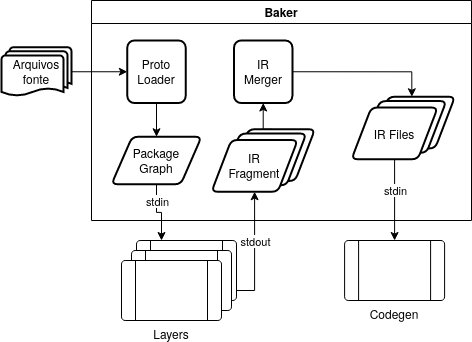
\includegraphics[width=0.8\linewidth]{Imagens/baker-diagram.png}
  \caption{Digrama do Fluxo de Dados do programa}
  \label{fig:baker-data-flow}
\end{figure}

\subsection{Comunicação Entre Programas}

Para permitir que os programas sejam escritos no maior número de linguagens de programação, a comunicação
entre o programa principal, \textit{layers} e \textit{codegens} é feita de forma similar a plugins para
\cite{googl:protobuf}: toda a comunicação é feita via entrada e saída padrão e utilizando Protocol Buffers
como formato. A saída padrão para erros é redirecionada para a saída padrão do programa como um todo, para
facilitar o relato de erros ao usuário.

O uso de Protocol Buffers ao invés de um formato customizado ou até mesmo JSON é devido a:

\begin{itemize}
\item Mantemos o padrão e simplificamos o fluxo.
\item Garante que as estruturas sejam construídas e geradas corretamente.
\item Facilita a manutenção de compatibilidade com \textit{layers} baseadas em versões anteriores
  da ferramenta.
\end{itemize}



% REFERENCIAS BIBLIOGRAFICAS
\renewcommand\bibname{\itareferencesnamebabel} %renomear título do capítulo referências
\bibliography{referencias}

\annex
\chapter{Exemplo em WSDL}\label{anex:wsdl-example}
\begin{minted}{xml}
<?xml version="1.0" encoding="UTF-8"?>
<description xmlns="http://www.w3.org/ns/wsdl"
             xmlns:tns="http://www.tmsws.com/wsdl20sample"
             xmlns:whttp="http://schemas.xmlsoap.org/wsdl/http/"
             xmlns:wsoap="http://schemas.xmlsoap.org/wsdl/soap/"
             targetNamespace="http://www.tmsws.com/wsdl20sample">

<documentation>
  This is a sample WSDL 2.0 document.
</documentation>

<!-- Abstract type -->
  <types>
    <xs:schema xmlns:xs="http://www.w3.org/2001/XMLSchema"
               xmlns="http://www.tmsws.com/wsdl20sample"
               targetNamespace="http://www.example.com/wsdl20sample">
     <xs:element name="Error" type="Error"/>
     <xs:element name="Pet" type="Pet"/>
     <xs:element name="Pets" type="Pets"/>
     <xs:element name="NewPet" type="NewPet"/>

     <xs:element name="ListPetsRequest" type="ListPetsRequest"/>
     <xs:element name="ShowPetByIdRequest" type="ShowPetByIdRequest"/>

     <xs:complexType name="Error">
      <xs:attribute name="code" type="xs:int"/>
      <xs:attribute name="message" type="xs:string"/>
     </xs:complexType>
     <xs:complexType name="Pet">
      <xs:attribute name="id" type="xs:int"/>
      <xs:attribute name="name" type="xs:string"/>
      <xs:attribute name="tag" type="xs:string" nillable="true"/>
     </xs:complexType>
     <xs:complexType name="NewPet">
      <xs:attribute name="name" type="xs:string"/>
      <xs:attribute name="tag" type="xs:string" nillable="true"/>
     </xs:complexType>
     <xs:complexType name="Pets">
      <xs:sequence>
        <xs:element minOccurs="0" name="pets" type="tns:Pet"/>
      </xs:sequence>
     </xs:complexType>

     <xs:complexType name="ListPetsRequest">
      <xs:attribute name="limit" type="xs:int" nillable="true"/>
      <xs:attribute name="cursor" type="xs:string" nillable="true"/>
     </xs:complexType>

     <xs:complexType name="ShowPetByIdRequest">
      <xs:attribute name="id" type="xs:int"/>
     </xs:complexType>
    </xs:schema>
  </types>

<!-- Abstract interfaces -->
  <interface name="PetStoreInterface">
    <fault name="Error1" element="tns:Error"/>
    <operation name="ListPets" pattern="http://www.w3.org/ns/wsdl/in-out">
      <input messageLabel="In" element="tns:ListPetsRequest"/>
      <output messageLabel="Out" element="tns:Pets"/>
    </operation>
    <operation name="CreatePet" pattern="http://www.w3.org/ns/wsdl/in-out">
      <input messageLabel="In" element="tns:NewPet"/>
      <output messageLabel="Out" element="tns:Pet"/>
    </operation>
    <operation name="ShowPetById" pattern="http://www.w3.org/ns/wsdl/in-out">
      <input messageLabel="In" element="tns:ShowPetByIdRequest"/>
      <output messageLabel="Out" element="tns:Pet"/>
    </operation>
  </interface>

<!-- Concrete Binding Over HTTP -->
  <binding name="HttpBinding" interface="tns:PetStoreInterface"
           type="http://www.w3.org/ns/wsdl/http">
    <operation ref="tns:ListPets" whttp:method="GET"/>
    <operation ref="tns:CreatePet" whttp:method="POST"/>
    <operation ref="tns:ShowPetById" whttp:method="GET"/>
  </binding>

<!-- Concrete Binding with SOAP-->
  <binding name="SoapBinding" interface="tns:PetStoreInterface"
           type="http://www.w3.org/ns/wsdl/soap"
           wsoap:protocol="http://www.w3.org/2003/05/soap/bindings/HTTP/"
           wsoap:mepDefault="http://www.w3.org/2003/05/soap/mep/request-response">
    <operation ref="tns:Get" />
    <operation ref="tns:CreatePet" />
    <operation ref="tns:ShowPetById" />
  </binding>

<!-- Web Service offering endpoints for both bindings-->
  <service name="PetStoreService" interface="tns:PetStoreInterface">
    <endpoint name="HttpEndpoint"
              binding="tns:HttpBinding"
              address="http://www.example.com/rest/"/>
    <endpoint name="SoapEndpoint"
              binding="tns:SoapBinding"
              address="http://www.example.com/soap/"/>
  </service>
</description>
\end{minted}


\chapter{Exemplo em OpenAPI}\label{anex:openapi-example}
\begin{minted}{yaml}
openapi: "3.0.0"
info:
  version: 1.0.0
  title: Swagger Petstore
  license:
    name: MIT
servers:
  - url: http://petstore.swagger.io/v1
paths:
  /pets:
    get:
      summary: List all pets
      operationId: listPets
      tags:
        - pets
      parameters:
        - name: limit
          in: query
          description: How many items to return at one time (max 100)
          required: false
          schema:
            type: integer
            format: int32
      responses:
        200:
          description: An paged array of pets
          headers:
            x-next:
              description: A link to the next page of responses
              schema:
                type: string
          content:
            application/json:
              schema:
                $ref: "#/components/schemas/Pets"
        default:
          description: unexpected error
          content:
            application/json:
              schema:
                $ref: "#/components/schemas/Error"
    post:
      summary: Create a pet
      operationId: createPets
      tags:
        - pets
      responses:
        201:
          description: Null response
        default:
          description: unexpected error
          content:
            application/json:
              schema:
                $ref: "#/components/schemas/Error"
  /pets/{petId}:
    get:
      summary: Info for a specific pet
      operationId: showPetById
      tags:
        - pets
      parameters:
        - name: petId
          in: path
          required: true
          description: The id of the pet to retrieve
          schema:
            type: string
      responses:
        200:
          description: Expected response to a valid request
          content:
            application/json:
              schema:
                $ref: "#/components/schemas/Pets"
        default:
          description: unexpected error
          content:
            application/json:
              schema:
                $ref: "#/components/schemas/Error"
components:
  schemas:
    Pet:
      required:
        - id
        - name
      properties:
        id:
          type: integer
          format: int64
        name:
          type: string
        tag:
          type: string
    Pets:
      type: array
      items:
        $ref: "#/components/schemas/Pet"
    Error:
      required:
        - code
        - message
      properties:
        code:
          type: integer
          format: int32
        message:
          type: string
\end{minted}


\chapter{Exemplo em Protocol Buffers}\label{anex:protobuf-example}
\begin{minted}{protobuf}
syntax = "proto3";

import "google/protobuf/empty.proto";

package petstore;

// Interface exported by the server.
service PetStoreService {
  // List all pets.
  rpc ListPets(ListPetsRequest) retuns (ListPetsResponse);

  // Create a pet.
  rpc CreatePet(CreatePetRequest) returns (google.protobuf.Empty);

  // Info for a specific pet.
  rpc ShowPetById(ShowPetByIdRequest) returns (Pet);
}

message ListPetsRequest {
  // How many items to return at one time (max 100).
  optional uint32 limit = 1;
  // A link to the page of responses
  optional string cursor = 2;
}

message ListPetsResponse {
  // A paged array of pets
  repeated Pet pets = 1;
  // A link to the next page of responses
  optional string cursor = 2;
}

message CreatePetRequest {
  string name = 2;
  optional string tag = 3;
}

message ShowPetByIdRequest {
  // The id of the pet to retrieve
  uint64 id = 1;
}

message Pet {
  uint64 id = 1;
  string name = 2;
  optional string tag = 3;
}
\end{minted}



% Glossario
%\itaglossary
%\printglossary

% Folha de Registro do Documento
% Valores dos campos do formulario
\FRDitadata{25 de março de 2015}
\FRDitadocnro{DCTA/ITA/DM-018/2015} %(o número de registro você solicita a biblioteca)
\FRDitaorgaointerno{Instituto Tecnológico de Aeronáutica -- ITA}
%Exemplo no caso de pós-graduação: Instituto Tecnol{\'o}gico de Aeron{\'a}utica -- ITA
\FRDitapalavrasautor{Cupim; Cimento; Estruturas}
\FRDitapalavrasresult{Cupim; Dilema; Construção}
%Exemplo no caso de graduação (TG):
\FRDitapalavraapresentacao{Trabalho de Graduação, ITA, São José dos Campos, 2015. \NumPenultimaPagina\ páginas.}
%Exemplo no caso de pós-graduação (msc, dsc):
%\FRDitapalavraapresentacao{ITA, São José dos Campos. Curso de Mestrado. Programa de Pós-Graduação em Engenharia Aeronáutica e Mecânica. Área de Sistemas Aeroespaciais e Mecatrônica. Orientador: Prof.~Dr. Adalberto Santos Dupont. Coorientadora: Prof$^\textnormal{a}$.~Dr$^\textnormal{a}$. Doralice Serra. Defesa em 05/03/2015. Publicada em 25/03/2015.}
\FRDitaresumo{Sistemas Web apresentam um grau de complexidade bastante diversificado, variando desde
um sistema comercial de um mercado de bairro até o sistema completo de uma multi-nacional
em escala global. Para simplificar o desenvolvimento desses sistemas, diversas ferramentas
foram desenvolvidas.

Este trabalho apresenta um novo modelo de gerador de APIs, com o objetivo de solucionar
problemas que ferramentas atuais apresentam. Esses problemas são relacionados a baixa
integração com outras ferramentas de desenvolvimento, como Object-Relational Mappings
(ORMs) e validadores. Mostramos também que o uso de um gerador que integre eficientemente
com o restante do ecossistema pode resultar em grandes ganhos de eficiência para o time de
desenvolvimento, além de abrir portas para o uso de outras ferramentas que não seriam possíveis
sem ele. Uma motivação para esse trabalho é a busca do aumento de eficiência e automação dentro
do processo de desenvolvimento e a redução na incidência de defeitos em sistemas complexos.
}
%  Primeiro Parametro: Nacional ou Internacional -- N/I
%  Segundo parametro: Ostensivo, Reservado, Confidencial ou Secreto -- O/R/C/S
\FRDitaOpcoes{N}{O}
% Cria o formulario
%\itaFRD


\end{document}

% Fim do Documento. O massacre acabou!!! :-)
